\problemname{Simply Sudoku}

Sudoku puzzles come in all different shapes and difficulty levels. Traditionally
a Sudoku puzzle is a $9\times9$ grid. Initially, some of the cells are filled in
with numbers and some are empty. The goal is to fill in each cell with a number
in the range $1$ -- $9$ subject to the following
restrictions:
\begin{itemize}
\item Each digit $1$ -- $9$ must appear once in each row
\item Each digit $1$ -- $9$ must appear once in each column
\item Each digit $1$ -- $9$ must appear once in each $3\times3$ sub-grid
\end{itemize}

The difficulty of a Sudoku puzzle can vary widely. The easiest puzzles can be solved with the following two simple techniques: \begin{description}
\item[Single Value Rule:] search for squares which only have one possible value that can be put there.
\item[Unique Location Rule:] within any row, column or sub-grid search for a value that can only be placed in one of the nine locations.
\end{description}
Consider the partially solved Sudoku puzzle shown in Figure \ref{fig1:example}.  The Single Value Rule applies to grid square A$7$ where $8$ is the only value that can be placed there.  The Unique Location Rule can be used to put a $5$ in square B$3$ as it is the only location in row $3$ where a $5$ can be placed.

\begin{figure}[h]
\centering
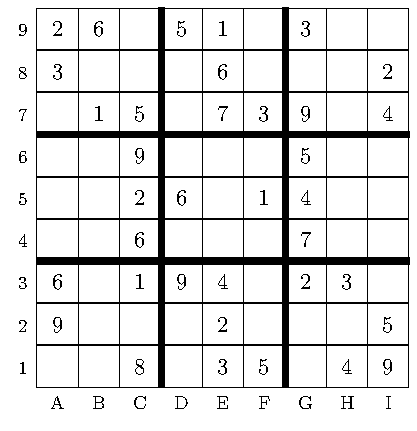
\includegraphics[width=0.5\textwidth]{sudoku-fig.pdf}
%\setlength{\unitlength}{2pt}
%\begin{picture}(100,100)(-10,-10)
%\put( 0, 0){\line(1,0){90}} \put(-5, 5){\makebox(0,0){$1$}}
%\put( 0,10){\line(1,0){90}} \put(-5,15){\makebox(0,0){$2$}}
%\put( 0,20){\line(1,0){90}} \put(-5,25){\makebox(0,0){$3$}}
%\put( 0,30){\line(1,0){90}} \put(-5,35){\makebox(0,0){$4$}}
%\put( 0,40){\line(1,0){90}} \put(-5,45){\makebox(0,0){$5$}}
%\put( 0,50){\line(1,0){90}} \put(-5,55){\makebox(0,0){$6$}}
%\put( 0,60){\line(1,0){90}} \put(-5,65){\makebox(0,0){$7$}}
%\put( 0,70){\line(1,0){90}} \put(-5,75){\makebox(0,0){$8$}}
%\put( 0,80){\line(1,0){90}} \put(-5,85){\makebox(0,0){$9$}}
%\put( 0,90){\line(1,0){90}}
%\put( 0, 0){\line(0,1){90}} \put( 5,-5){\makebox(0,0){A}}
%\put(10, 0){\line(0,1){90}} \put(15,-5){\makebox(0,0){B}}
%\put(20, 0){\line(0,1){90}} \put(25,-5){\makebox(0,0){C}}
%\put(30, 0){\line(0,1){90}} \put(35,-5){\makebox(0,0){D}}
%\put(40, 0){\line(0,1){90}} \put(45,-5){\makebox(0,0){E}}
%\put(50, 0){\line(0,1){90}} \put(55,-5){\makebox(0,0){F}}
%\put(60, 0){\line(0,1){90}} \put(65,-5){\makebox(0,0){G}}
%\put(70, 0){\line(0,1){90}} \put(75,-5){\makebox(0,0){H}}
%\put(80, 0){\line(0,1){90}} \put(85,-5){\makebox(0,0){I}}
%\put(90, 0){\line(0,1){90}}
%\put( 5,15){\makebox(0,0){$9$}}
%\put( 5,25){\makebox(0,0){$6$}}
%\put( 5,75){\makebox(0,0){$3$}}
%\put( 5,85){\makebox(0,0){$2$}}
%
%\put(15,65){\makebox(0,0){$1$}}
%\put(15,85){\makebox(0,0){$6$}}
%
%\put(25, 5){\makebox(0,0){$8$}}
%\put(25,25){\makebox(0,0){$1$}}
%\put(25,35){\makebox(0,0){$6$}}
%\put(25,45){\makebox(0,0){$2$}}
%\put(25,55){\makebox(0,0){$9$}}
%\put(25,65){\makebox(0,0){$5$}}
%
%\put(35,25){\makebox(0,0){$9$}}
%\put(35,45){\makebox(0,0){$6$}}
%\put(35,85){\makebox(0,0){$5$}}
%
%\put(45, 5){\makebox(0,0){$3$}}
%\put(45,15){\makebox(0,0){$2$}}
%\put(45,25){\makebox(0,0){$4$}}
%\put(45,65){\makebox(0,0){$7$}}
%\put(45,75){\makebox(0,0){$6$}}
%\put(45,85){\makebox(0,0){$1$}}
%
%\put(55, 5){\makebox(0,0){$5$}}
%\put(55,45){\makebox(0,0){$1$}}
%\put(55,65){\makebox(0,0){$3$}}
%
%\put(65,25){\makebox(0,0){$2$}}
%\put(65,35){\makebox(0,0){$7$}}
%\put(65,45){\makebox(0,0){$4$}}
%\put(65,55){\makebox(0,0){$5$}}
%\put(65,65){\makebox(0,0){$9$}}
%\put(65,85){\makebox(0,0){$3$}}
%
%\put(75, 5){\makebox(0,0){$4$}}
%\put(75,25){\makebox(0,0){$3$}}
%
%\put(85, 5){\makebox(0,0){$9$}}
%\put(85,15){\makebox(0,0){$5$}}
%\put(85,65){\makebox(0,0){$4$}}
%\put(85,75){\makebox(0,0){$2$}}
%\thicklines
%\put( 0,30){\line(1,0){90}}
%\put( 0,60){\line(1,0){90}}
%\put(30, 0){\line(0,1){90}}
%\put(60, 0){\line(0,1){90}}
%\end{picture}
\caption{Sample Input $1$}
\label{fig1:example}
\end{figure}
The easiest Sudoku puzzles can be solved with only these two rules; harder puzzles use techniques like swordfish, x-wings and BUGs.

For this problem you will be given a Sudoku puzzle and must determine if it is an easy puzzle, i.e., whether it can be solved by just using the Single Value and Unique Location rules.

\section*{Input}
Input consists of a single Sudoku puzzle given over nine lines.  Each line contains $9$ values in the range $0$ to $9$, where a $0$ indicates a blank in the puzzle.

\section*{Output}
Output the word {\tt Easy} followed by the solved Sudoku puzzle if it is an easy puzzle.  The puzzle should be printed on nine lines with a single space separating values on a line.  If the puzzle is not easy output {\tt Not easy} followed by as much of the Sudoku puzzle as can be solved using the two rules described above.  Use the same format for the partial solution as for the complete solution using a `{\tt .}' instead of a digit for a unfilled square.
